%Linea Para poder completar automaticamente las citas con el Sublime
%No hace el documento, se puede borrar esta linea si no se usa el Sublime
%------------------------------------------------------------------------------
 \newcommand{\NoBiblioConc}[1]{
 \ifthenelse{\equal{#1}{verdadero}}{}{\bibliography{Referencias/base_bibliografica}}
 \NoBiblioConc{verdadero}}
 %-----------------------------------------------------------------------------

%Formato (Nombre de capitulo largo o corto), nombre del capitulo y estilo de la
%Portada del Capitulo
%------------------------------------------------------------------------------
 	
 %Formato en si, titulo en un solo renglon
 \FormatoCapituloUnaLinea
 
 %Nombre y etiquete para referir
 \chapter{Conclusiones}
 \label{chap:Conclusiones}

 %Para que no salga el numero de pagina en la portada del capitulo
 \thispagestyle{empty}
	
 %Resumen del Capitulo en Italica


 %Indice de capitulo alineada al borde inferior de la pagina, nueva pagina
 \vfill
 \minitoc
 \newpage
 %-------------------------------------------------------------------------------

\section{Conclusiones Generales}

 A lo largo de la tesis toda la concentración y el esfuerzo estuvieron dedicados a la fabricación escalable de multisensores electroquímicos permeoselectivos. 

 Las primeras etapas tuvieron como eje la compatibilidad entre los procesos de fabricación \textit{top-down} y \textit{bottom-up}. Los primeros para diseñar, fabricar y evaluar el despempeño electroquímico de los electrodos de Au de los multisensores y los segundos, para sintetizar las películas delgadas mesoporosas de diferentes tamaños de poros utilizando diferentes surfactante (Pluronic F127, Brij58 y CTAB). Las problemáticas que allí surgieron estuvieron vinculadas a la pobre adherencia de las películas delgadas mesoporosas a los electrodos y a las temperaturas de calcinación usadas tradicionalmente para condensar y eliminar el molde en dichas películas. La solución a los problemas de adherencia se basó realizar modificaciones superficiales sobre los electrodos utilizando moléculas de anclaje químicamente compatible con las películas de SiO$_2$. La temperatura de calcinación, típicamente $\geq$\SI{350}{\celsius} favorece los procesos difusivos de impurezas hacia la superficie de los electrodos, afectando el desempeño electroquímico de los sensores. Con el objetivo de mantener la calidad analítica de los electrodos se plantearon dos estrategias: 1) fabricar los multisensores vía calcinación pero sobre electrodos de Au de mayor pureza, libre de cantidades significativas de impurezas y, 2) disminuir la temperatura de condensación de las películas mesoporosas de SiO$_2$ hasta \SI{130}{\celsius} a fin de minimizar los procesos difusivos y disminuir sensiblemente la concentración de impurezas en superficie. La primera, más simple de implementar, fue la que primero se llevo a cabo obteniéndose resultados satisfactorios. Sin embargo, la segunda era la que presentaba mayores desafíos tanto científicos como tecnológicos. Se requería estabilizar la estructura del cristal líquido, condensar el óxido manteniendo la temperatura por debajo de \SI{130}{\celsius}, extraer el surfactante y mantener el buen desempeño electroquímico de los electrodos.  

 Tomando algunos aspectos de la literatura especializadas se llevaron a cabo métodos novedosos para la condensación de las películas y eliminación del molde. Para este fin se diseñaron y experimentaron cinco procesos posdepósito: simplificado, prolongado, ácido, alcalino y alto vacío. Todo el capítulo 3 está dedicado a la comparación de las propiedades y características de las películas delgadas mesoporosas obtenidas por estos procesos con las obtenidos por el método clásico de calcinación. Las caracterizaciones incluyeron técnicas como elipsoporosimetría ambiental, microscopía óptica, de barrido electrónico y de iones focalizados de galio, espectroscopía IR, ángulo de contacto y voltametría cíclica. Se evaluaron características como índice de refracción, espesor, grado de condensación, grado de extracción del surfactante, accesibilidad, porosidad y distribución de tamaño de poros y cuellos. Todos los métodos llevaron a películas porosas con características distintivas que se detallan y discuten en dicho capítulo. A pesar de que se podría haber usado cualquiera de los procesos desarrollados, se consideró el método de alto vacío el más adecuado para avanzar hacía la elaboración de multisensores electroquímicos selectivos. Esta elección esta fundamentada en que el método de alto vacío fue el proceso que mostró películas con propiedades equivalentes a las calcinadas y, además, no utiliza reactivos extra en la síntesis, lo que redunda en una síntesis limpia, libre de interferentes, productos de reacciones secundarias o moléculas sensibles de ser adsorbidas. El desarrollo de estos métodos no sólo permitió minimizar los procesos difusivos, obtener respuestas electroquímicas de calidad sino que también abre el camino para depositar películas mesoporosas de óxidos puros o mixtos sobre sustratos térmicamente lábiles, como acrílicos, PET o polímeros en general.

 Durante todo el trabajo de tesis, las mediciones electroquímicas fueron una labor que se llevó en forma transversal y constante. Los resultados de las mismas está distribuidas a lo largo de todos lo capítulos de la tesis. Estas tuvieron gran relevancia y múltiples propósitos: 1) evaluar el desempeño electroquímico de las películas delgadas de (Cr,Ti)\textbar Au destinadas a usar como electrodos, 2) comprobar la accesibilidad de moléculas dentro de las películas delgadas mesoporosas, 3) estudiar los mecanismos de transporte y obtener parámetros fisicoquímicos de los sistemas porosos, y 4) medir analíticamente la respuesta de las sondas en un multisensor conformado con electrodos de diferentes características.

 El análisis minucioso y sistemático sobre los voltagramas, tanto de corriente continua como de corriente alterna, llevaron a conclusiones generales sobre el transporte de moléculas dentro de los poros. Se utilizaron sondas electroactivas de distinta carga: \ferroferri\space de carga negativa, \aminorutenio\space de carga positiva y \ferroceno\space de carga neutra. Los resultados obtenidos permitieron evaluar las propiedades permeoselectivas de las membranas y, a su vez, establecer la capacidad de preconcentración, estimar la concentración de sonda adsorbida, proponer un mecanismo para el transporte de carga dentro de las películas y calcular coeficientes de difusión tanto para la permeación ($D$) como para la transferencia de carga mediante \textit{electron hopping} ($D_e$).Se realizaron simulaciones por el método de elementos finitos y experimentos electroquímicos con el ánimo de establecer bajo qué condiciones de contorno se pueden manifestar fenómenos de mediación rédox entre una película saturada con un mediador y un analito en solución. No fue posible reproducir experimentalmente dichas condiciones, sin embargo se realizaron simulaciones con posibles escenarios, y a partir de estos experimentos, se realizó un análisis profundo de cómo influyen la constante de difusión $D_e$ y la constante de equilibrio $K$ en demérito de dicho proceso de mediación. 

 Un resultado relevante para la aplicación de películas delgadas mesoporosas de SiO$_2$ en sensores permeoselectivos, fue la demostración de la disolución de las mismas  catalizada por el ciclado electroquímico. Se depositaron soles agregando un 10\% en masa de ZrCl$_4$ en su formulación, seguidas por el tratamiento en alto vacío lo que llevó a películas mesoporosasa homogéneas de composición general Si$_{0.9}$Zr$_{0.1}$O$_2$. La adición de Zr permitió aumentar la estabilidad química y mecánica de las películas manteniendo las propiedades permeoselectivas y sin perder capacidad de adsorción de \aminorutenio. Con la intención de regular las propiedades de transporte se funcionalizaron estas películas, de gran estabilidad, con dihexadecilfosfato (DHDP) y 3-aminopropil trietoxisilano (APTES). Se discutieron e interpretaron cómo se afecta el transporte debido a estas funcionalizaciones; llegando a la conclusión de que la cinética y la capacidad de adsorción, en particular para \ru, se ven significativamente afectadas. Si bien los sistemas permeoselectivos estudiados comprendieron películas delgadas mesoporosas de SiO$_2$ y Si$_{0.9}$Zr$_{0.1}$O$_2$ con sondas modelo con carga positiva, negativa y neutra, las interpretaciones y conclusiones que se desprendieron de este trabajo (en particular las referentes a  fenómenos y dinámica de transporte) pueden ser aplicados a sistemas donde se modifiquen las condiciones de permeoseletividad debido a películas con un mayor IEP (p. ej. TiO$_2$ o ZrO$_2$) o funcionalizadas con polielectrolitos. 
 
 Se fabricaron multisensores recurrentemente a lo largo de todo el período que llevó el trabajo. Se hizo primero un diseño que luego fue reemplazado por uno más compacto y especialmente optimizado para usar en procesos electroquímicos. En esta última etapa se volcó toda la experiencia adquirida para fabricar electrodos de Ti\textbar Au recubiertos con películas de mixtas Si$_{0.9}$Zr$_{0.1}$O$_2$ con poros de \SI{\approx 9}{\nm} de diámetro, sintetizadas por el método de alto vacío para mantener la calidad analítica de los electrodos. Finalmente se funcionalizaron las películas con DHDP y APTES sobre algunos de ellos, con el próposito de obtener un multisensor prototipo con cuatro electrodos de características diferentes. Sobre este prototipo se llevaron a cabo mediciones electroquímicas para cada una de las sondas de distinta carga: \ferroferri, \ferroceno\space y \aminorutenio. Las múltiples respuestas electroquímicas obtenidas se analizaron con gráficos radiales a lo largo de un determinado tiempo de medición con el fin de obtener una marca sensorial para cada una de las sondas, las cuales indican de forma fácilmente observable, si hay exclusión, permeación o la cantidad de sonda adsorbida. Estas marcas sensoriales pueden ser de gran utilidad como elemento distintivo a modo de <<huella digital>> para clasificar familias de compuestos, clasificar comportamientos de grupos de analitos o directamente identificar de forma rápida, \textit{in situ} y a bajo costo aquellos compuestos con marcas sensoriales específicas.

 Los novedosos métodos posdepósito y el refuerzo dado por la adición de circonio a las películas delgadas mesoporosas, sumado al meticulosos estudio electroquímico y al análisis de sensado multivariable que se presentó en este trabajo abrirán caminos poco explorados hasta el momento, pero con gran potencial en el campo de los sensores electroquímicos basados en materiales mesoporosos.

\section{Perspectivas para futuros trabajos}
 
 		El presente trabajo presenta al menos dos líneas claramente definida para continuar con desarrollos e investigaciones en el área. La primera relacionada al estudio de la fisicoquímica en espacios confinados, transporte y cinética de adsorción/desorción por citar algunos ejemplos; y la segunda, relacionada con aplicaciones y desarrollo en sensores, propiedades permeoselectivas, marcas sensoriales especificas para distintos analitos de interés y desarrollo de métodos de análisis multivariable entre otros.
 
 		Esta sección tiene por motivación mostrar y ejemplificar muy brevemente algunos experimentos, ideas y pruebas de concepto que se llevaron a cabo paralelamente al eje central de esta tesis. No es el propósito de este apartado realizar demostraciones formales o hacer discusiones profundas de los resultados, sino presentar algunos avances y experimentos conceptuales surgidos de los conocimientos y experiencia adquiridas durante esta tesis con perspectivas a futuros desarrollos e investigaciones.
  
  \subsection{Integración en circuitos integrados}

	  La ventaja de fabricar electrodos por técnicas de microelectrónica es indiscutible. Existen muchas fábricas a nivel global de microsistemas (MEMS) y circuitos integrados (IC) (conocidas en ingles simplemente como \textit{foundry}). Dichas fabricadas elaboran sus productos con procesos estándar de fabricación por cada nodo tecnológico, con reglas de diseño claras, bien establecidas y con sistemas de depuración de errores. La integración de sensores en circuitos integrados no es algo nuevo, y, dado el nivel de integración de la electrónica de las últimas décadas, es algo que siempre se debe tener en cuenta en la etapa de prototipado de sensores.\cite{Wang2012,Liu1993,Novell2012,Yu2013,Sarkar2014} El desarrollo y optimización de los procesos para depositar \pdm\space a bajas temperaturas simplifica la posibilidad de incorporar los multisensores y un potenciostato en un microchip, incorporando a su vez en la lógica del circuito integrado algoritmos para el análisis multivariable.

	  El INTI cuenta con un equipo de profesionales dedicados al diseño de IC, con experiencia en diseñar potenciostatos dedicados, integrados completamente en silicio e ideados para aplicaciones \textit{ad hoc}\cite{sanmartin2011}. A diferencia de los potenciostatos de mesada, los integrados en microchip cuenta con varias ventajas: el bajo costo de fabricación, la portabilidad y la natural comunicación con dispositivos móviles como celulares, tabletas o notebooks.\cite{longinotti2010,Salomon2014} En la figura \ref{fig:pote-onchip} se muestra un potenciostato fabricado en un circuito integrado codiseñado entre el INTI y la UNSAM (Universisdad Nacional de San Martín), el cual fue fabricado específicamente para un dispositivo electroquímico portable para detección de enfermedades infecciosas \cite{Kuo2018}.	 
 			
 			\begin{figure}[th!]
			    \begin{center}
			    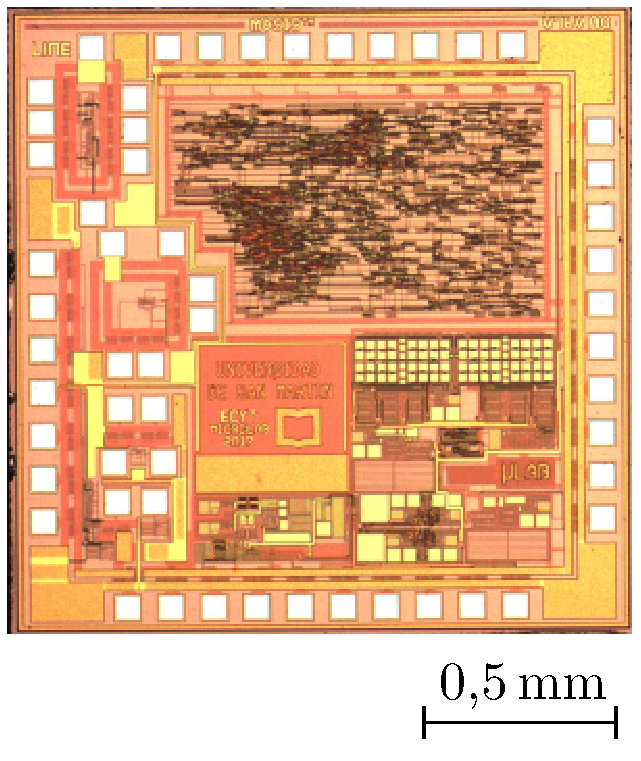
\includegraphics[width=0.72\textwidth]{Imagenes/potenciostato-chip.pdf}
	       		\caption{Microscopía óptica de un circuito integrado el cual incorpora un potenciostato. Diseñado en conjunto entre INTI y UNSAM y fabricado por la empresa \textit{The MOSIS Service}. Forma parte de un dispositivo electroquímico para la detección de enfermedades infecciones para ser utilizado tanto en humanos como en sanidad animal.}
	         	\label{fig:pote-onchip}
	     		\end{center}
	     		\end{figure}

  \subsection{Multisensores impresos}

  			\begin{figure}[b!]
			 	   	    \centering
			 	   	    \begin{subfigure}[t]{0.495\textwidth}
			        	\includegraphics[width=\textwidth]{Imagenes/Inkjet-02-escala-fondo.jpg}
			        	\caption{\pdmF\space impresos sobre oblea de silicio. Recuadro: MEB donde se observa la estructura porosa.}
			       		\end{subfigure}
			     		\centering
			     		\begin{subfigure}[t]{0.495\textwidth}
			     		\includegraphics[width=0.85\textwidth]{Imagenes/Inkjet-05-escala-fondo.jpg}
			    		\caption{\pdmF\space impresos sobre oblea de silicio con un depósito de Ti\textbar Au.}
			    		\end{subfigure}
			    		\centering
			    		\begin{subfigure}[t]{0.495\textwidth}
			         	\includegraphics[width=0.80\textwidth]{Imagenes/Inkjet-04-escala-fondo.jpg}
			        	\caption{\pdmF\space impresos sobre microelectrodos.}
			        	\end{subfigure}
			        	\centering
			        	\begin{subfigure}[t]{0.495\textwidth}
			     		\includegraphics[width=\textwidth]{Imagenes/Inkjet-03-escala-fondo.jpg}
 			        	\caption{\pdmF\space impresos en Ti\textbar	Au en soporte de poliestireno de alto impacto.}
			        	\end{subfigure}
			     		\caption[Electrodos impresos]{Fotografías de películas mesoporosas de SiO$_2$ impresas por inyección de tinta a partir de soles modificados y diseños arbitrarios. Los poros fueron moldeados con F127 y la condensación se realizó por el método de alto vacío. La extracción se llevó a cabo con 2-propanol y agua a pH=2.}
			     		\label{fig:flexibles}
			     	   	\end{figure}

 	  Otro aspecto que se trabajó durante este trabajo es la posibilidad de transferir diseños arbitrarios a las películas mesoporosas. Existen antecedentes en la literatura dónde ya han trabajado estos aspectos mediante diversos métodos: litografía con luz UV, litografía con rayos X, microscopía de fuerza atómica, electroquímica, impresión vía chorro de tinta, etc.\cite{Innocenzi2008}. 

 	  Habiendo grupos de investigación en el INTI que trabajan en el desarrollo de tintas para la industria electrónica, se optó por el método de impresión para la transferencia de diseños. Se usaron soles levemente modificados para las tintas y se imprimieron sobre diversos sustratos, además, de esta forma se podrían imprimir \pdm\space de igual o distintos óxidos en un mismo sustrato. Se trabajó en colaboración con el grupo del Dr. Baumann, del \textit{Department of Digital Printing and Imaging Technology} de la \textit{Technische Universität Chemnitz} de Alemania (\url{https://www.tu-chemnitz.de/mb/DigiTech/professorship.php}). Allí imprimieron soles modificados con etilenglicol en un equipo de inyección de tinta sobre una amplia variedad de sustratos. Los procesos a baja temperatura desarrollados en este trabajo, no solo hacen que disminuya la difusión entre las capas metálicas, permitiendo la integración en microchips de silicio, sino que permite depositar las \pdm\space sobre sustratos térmicamente menos estables. Los resultados fueron sistemas porosos de soles de SiO$_2$, estructurados con F127 impresos sobre silicio, oro, microelectrodos y poliestireno de alto impacto (PAI). Se muestran, en la figura \ref{fig:flexibles}, patrones cuadrados impresos sobre una diversidad de sustratos variando los parámetros de impresión, con el objetivo de encontrar las condiciones óptimas para una correcta transferencia.

 	  Con la expectativa de poder realizar todo el proceso de fabricación de los multisensores con técnicas de impresión, se muestran en la figura \ref{fig:tintas}, electrodos impresos por inyección con tintas a base a nanotubos de carbono desarrolladas en el INTI-CMNB. Actualmente estas tintas están en desarrollo y en proceso de optimización para uso en sensores electroquímicos y enzimáticos\cite{longinotti2010,Mass2016}. En el panel de la derecha de la figura \ref{fig:tintas} se muestra la respuesta electroquímica para \fe\space \SI{2.5}{\milli\Molar}, si bien no es la misma que en electrodos de Au, es una respuesta reproducible y confiable, con un enorme potencial para depositar óxidos mesoporosos sobre su superficie. Se prevé próximamente imprimir ambos componentes en un solo sustrato y en un único proceso, los electrodos basados en tintas de nanotubos de carbono y las películas delgadas mesoporosas de óxidos mixtos silicio/circonio.

 	  			\begin{figure}[h!]
		 	   	    \begin{subfigure}[t]{0.25\textwidth}
			       	\includegraphics[width=\textwidth]{Imagenes/NTC1-fondo.jpg}
			   		\end{subfigure}
			   		\begin{subfigure}[t]{0.25\textwidth}
			       	\includegraphics[width=\textwidth]{Imagenes/NTC2-fondo.jpg}
			   		\end{subfigure}
			   		\begin{subfigure}[t]{0.43\textwidth}
			   	    \includegraphics[width=\textwidth]{Graficos/TintaNTC-FeCN2-5mM.pdf}
			   		\end{subfigure}
					 \caption[Electrodos de NTC flexibles.]{Electrodos basados en nanotubos de carbono impresos por inyección de tinta en  donde se muestra la flexibilidad de la tinta y su respuesta electroquímica con una sonda de \fe\space \SI{2.5}{\milli\Molar} en solución de KCl \SI{100}{\milli\Molar} a \SI{50}{\milli\volt\per\second}.}
					 \label{fig:tintas}	
				     \end{figure}

